\TODO

\section{Functionality}

\TODO

\section{Performance}

\TODO

\section{Fitness}

\TODO

\section{Example}

\todo{make into chapter?}

\begin{itemize}
    \item 21 rules and 13 states.
    \item Green goes in circle to form border, red when complete (but not corners).
    \item Cyan detaches from corners to form new circles.
    \item X to the right, Y upwards.
\end{itemize}

\begin{figure}[!ht]
    \centering
    \begin{subfigure}{0.32\textwidth}
        \centering
        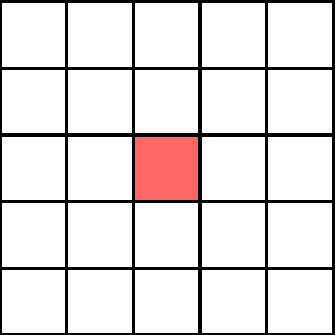
\includegraphics[width=0.9\textwidth]{replicator-1/00}
        \caption{Step 0}
    \end{subfigure}
    \begin{subfigure}{0.32\textwidth}
        \centering
        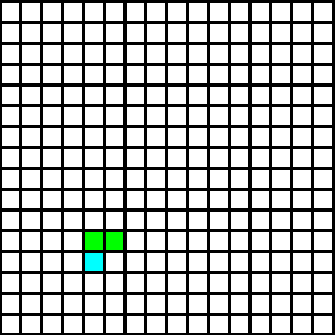
\includegraphics[width=0.9\textwidth]{replicator-1/01}
        \caption{Step 1}
    \end{subfigure}
    \begin{subfigure}{0.32\textwidth}
        \centering
        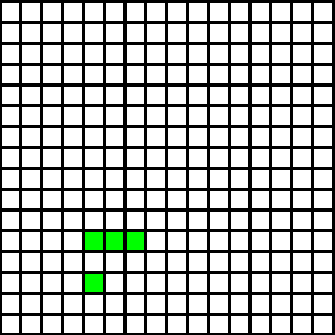
\includegraphics[width=0.9\textwidth]{replicator-1/02}
        \caption{Step 2}
    \end{subfigure}
    \begin{subfigure}{0.32\textwidth}
        \centering
        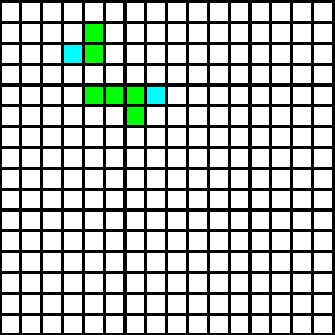
\includegraphics[width=0.9\textwidth]{replicator-1/03}
        \caption{Step 3}
    \end{subfigure}
    \begin{subfigure}{0.32\textwidth}
        \centering
        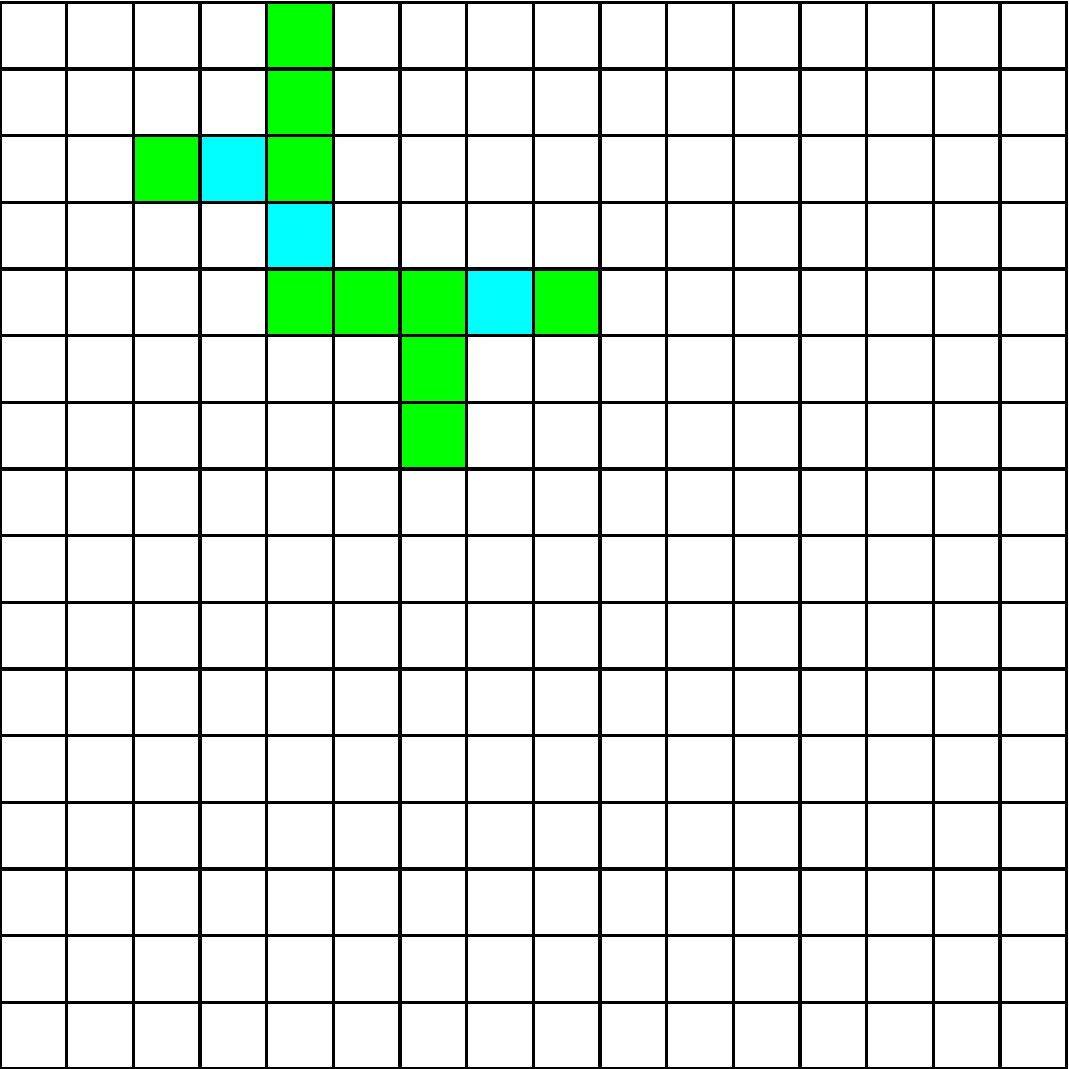
\includegraphics[width=0.9\textwidth]{replicator-1/04}
        \caption{Step 4}
    \end{subfigure}
    \begin{subfigure}{0.32\textwidth}
        \centering
        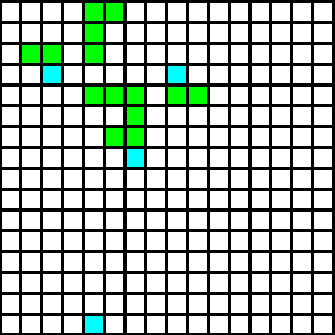
\includegraphics[width=0.9\textwidth]{replicator-1/05}
        \caption{Step 5}
    \end{subfigure}
    \begin{subfigure}{0.32\textwidth}
        \centering
        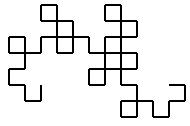
\includegraphics[width=0.9\textwidth]{replicator-1/06}
        \caption{Step 6}
    \end{subfigure}
    \begin{subfigure}{0.32\textwidth}
        \centering
        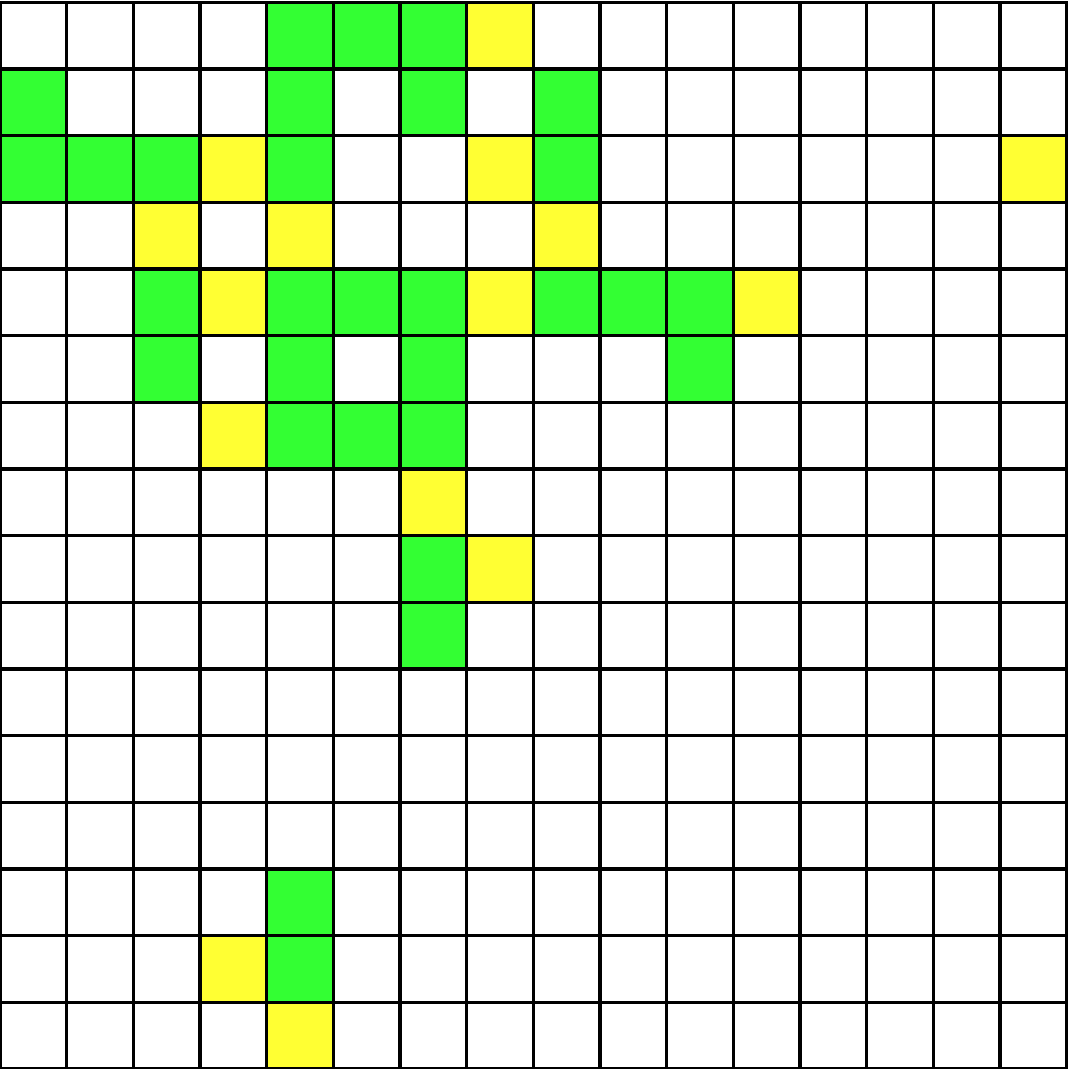
\includegraphics[width=0.9\textwidth]{replicator-1/07}
        \caption{Step 7}
    \end{subfigure}
    \begin{subfigure}{0.32\textwidth}
        \centering
        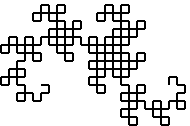
\includegraphics[width=0.9\textwidth]{replicator-1/08}
        \caption{Step 8}
    \end{subfigure}
    \begin{subfigure}{0.32\textwidth}
        \centering
        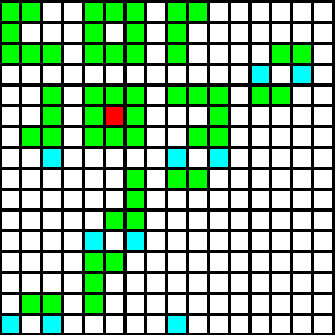
\includegraphics[width=0.9\textwidth]{replicator-1/09}
        \caption{Step 9}
    \end{subfigure}
    \begin{subfigure}{0.32\textwidth}
        \centering
        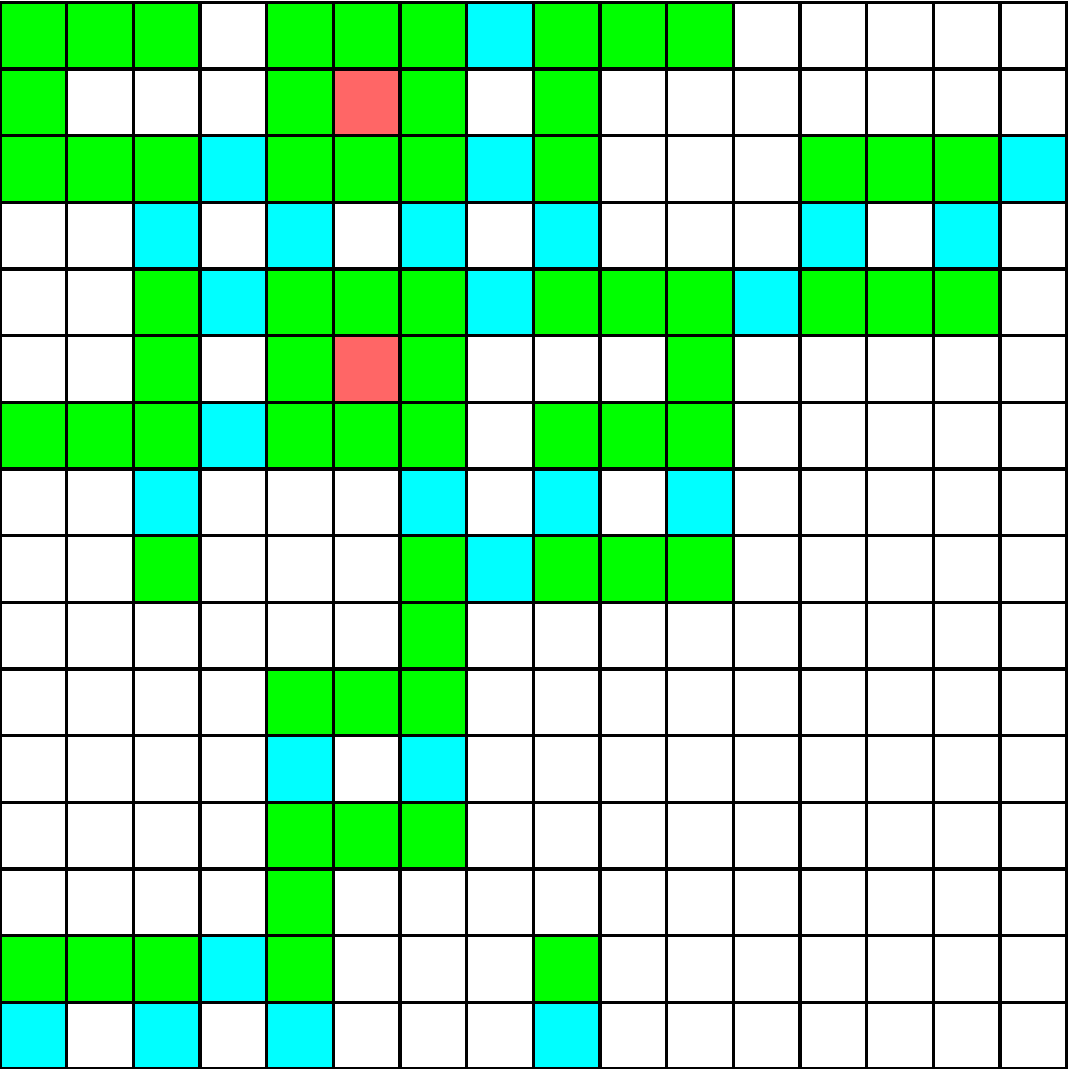
\includegraphics[width=0.9\textwidth]{replicator-1/10}
        \caption{Step 10}
    \end{subfigure}
    \begin{subfigure}{0.32\textwidth}
        \centering
        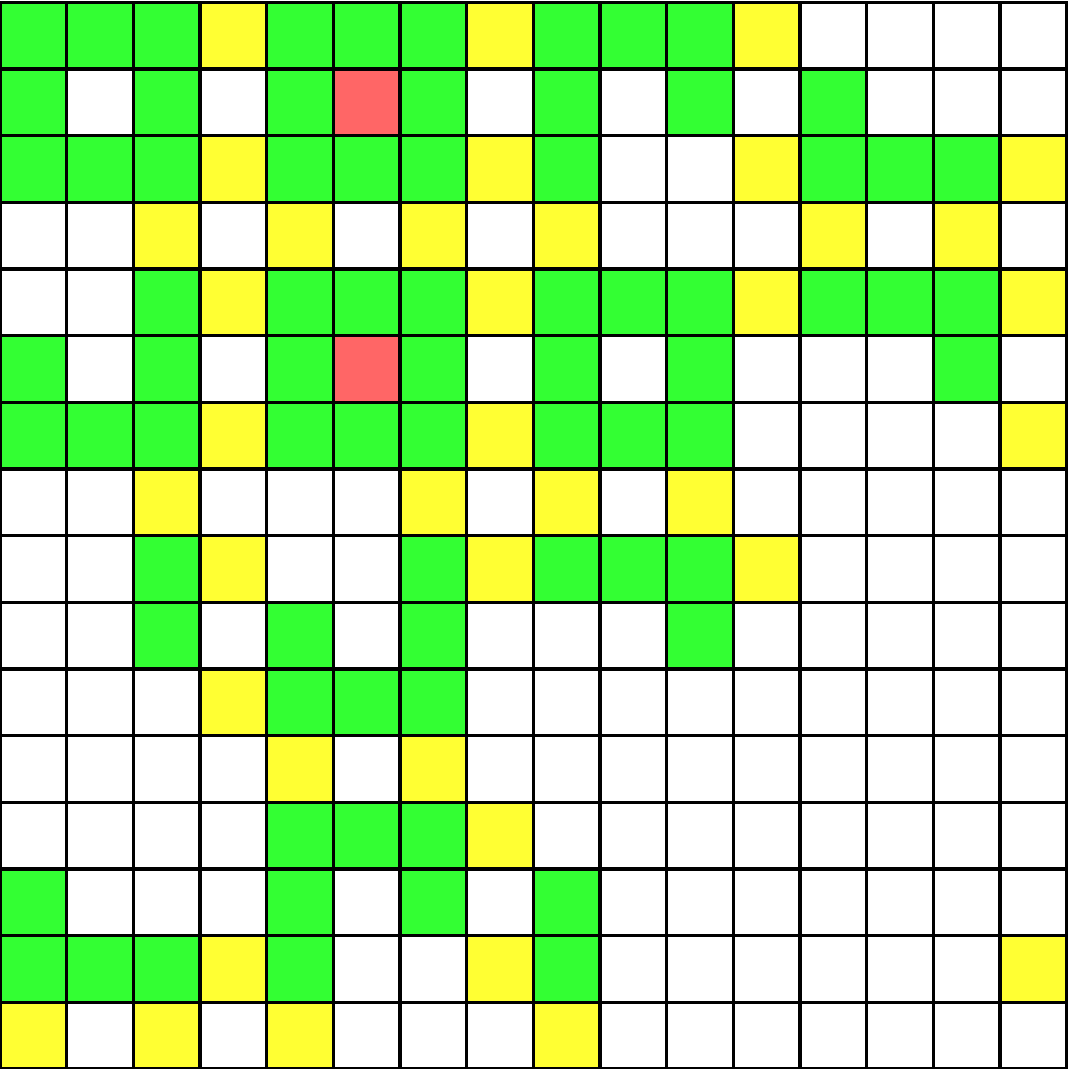
\includegraphics[width=0.9\textwidth]{replicator-1/11}
        \caption{Step 11}
    \end{subfigure}
\end{figure}

\begin{figure}[!ht]
    \ContinuedFloat
    \centering
    \begin{subfigure}{0.32\textwidth}
        \centering
        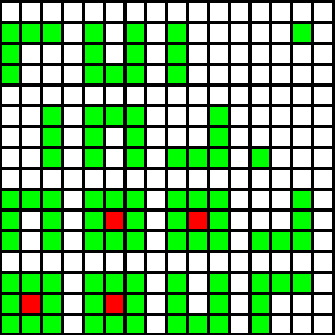
\includegraphics[width=0.9\textwidth]{replicator-1/12}
        \caption{Step 12}
    \end{subfigure}
    \begin{subfigure}{0.32\textwidth}
        \centering
        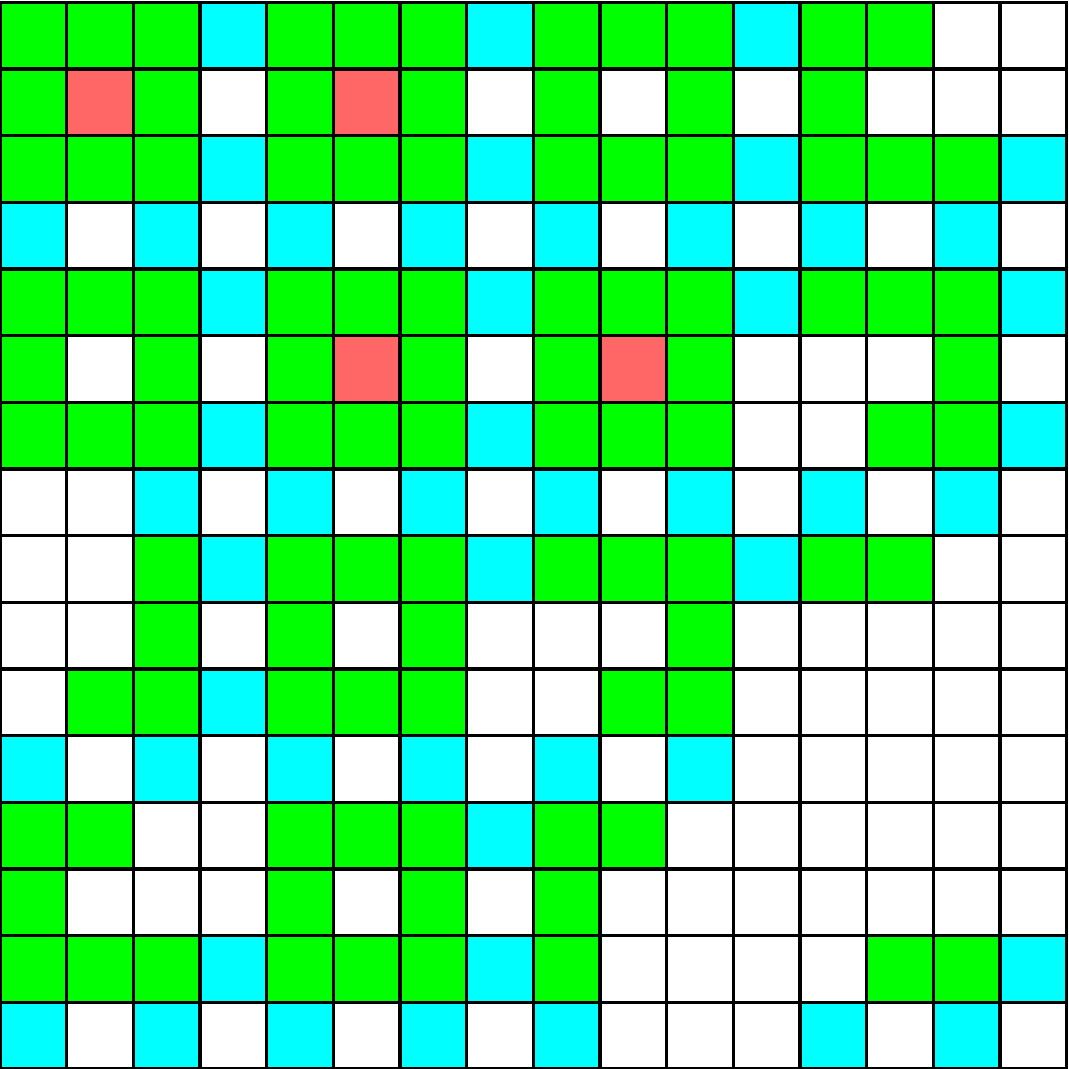
\includegraphics[width=0.9\textwidth]{replicator-1/13}
        \caption{Step 13}
    \end{subfigure}
    \begin{subfigure}{0.32\textwidth}
        \centering
        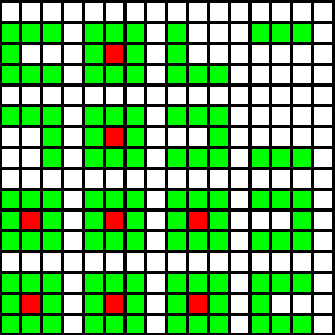
\includegraphics[width=0.9\textwidth]{replicator-1/14}
        \caption{Step 14}
    \end{subfigure}
    \begin{subfigure}{0.32\textwidth}
        \centering
        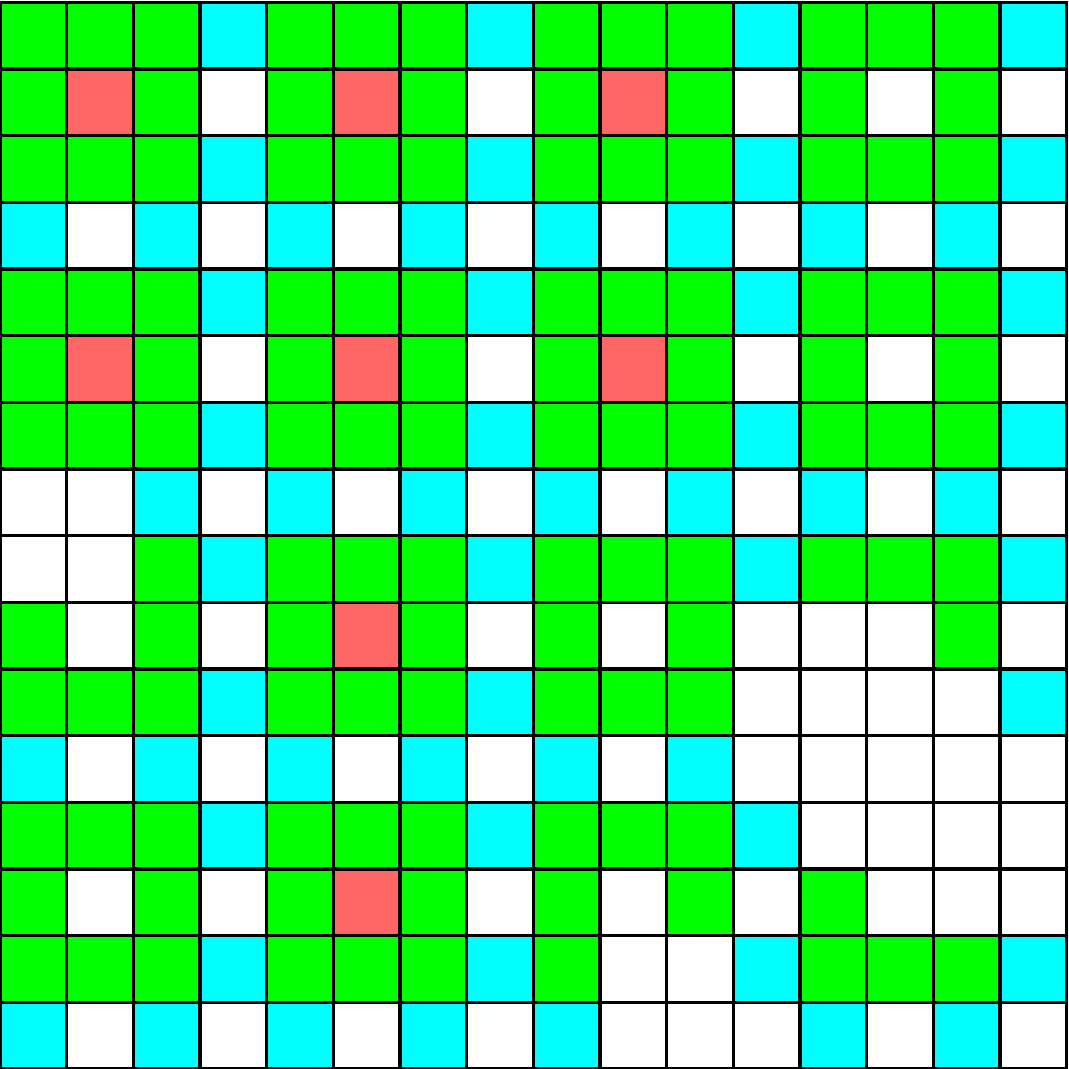
\includegraphics[width=0.9\textwidth]{replicator-1/15}
        \caption{Step 15}
    \end{subfigure}
    \begin{subfigure}{0.32\textwidth}
        \centering
        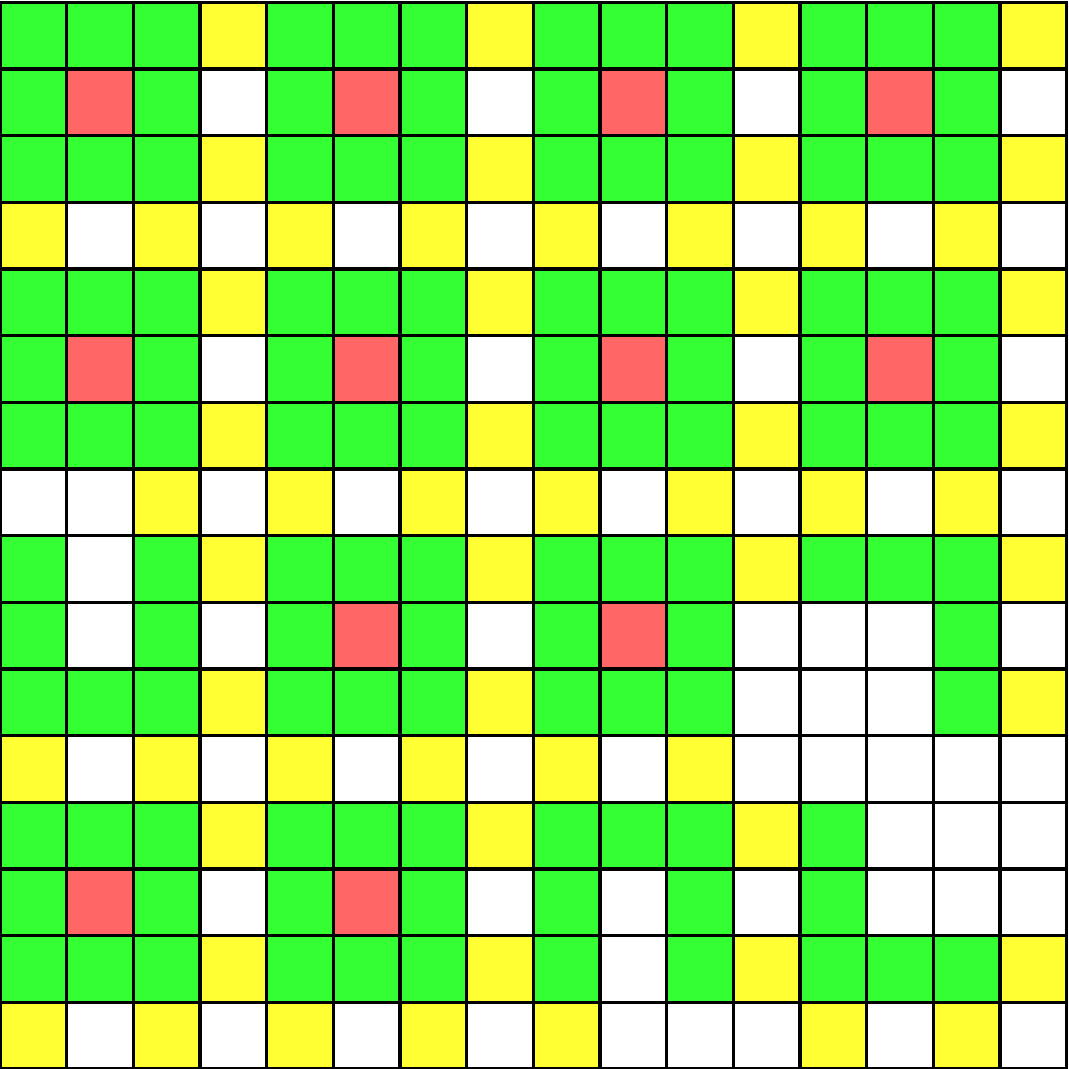
\includegraphics[width=0.9\textwidth]{replicator-1/16}
        \caption{Step 16}
    \end{subfigure}
    \begin{subfigure}{0.32\textwidth}
        \centering
        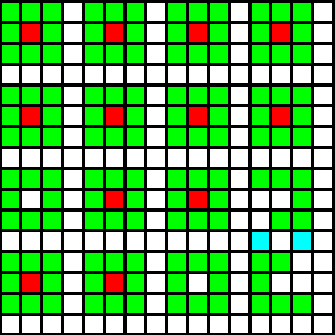
\includegraphics[width=0.9\textwidth]{replicator-1/17}
        \caption{Step 17}
    \end{subfigure}
    \begin{subfigure}{0.32\textwidth}
        \centering
        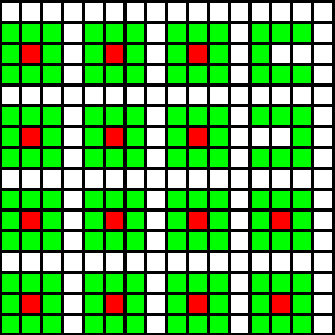
\includegraphics[width=0.9\textwidth]{replicator-1/18}
        \caption{Step 18}
    \end{subfigure}
    \begin{subfigure}{0.32\textwidth}
        \centering
        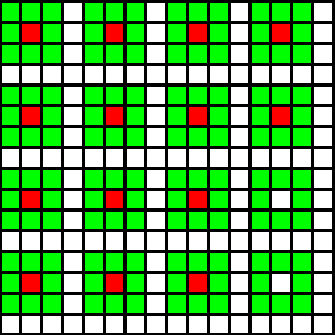
\includegraphics[width=0.9\textwidth]{replicator-1/19}
        \caption{Step 19}
    \end{subfigure}
    \begin{subfigure}{0.32\textwidth}
        \centering
        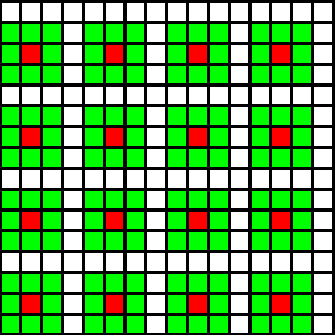
\includegraphics[width=0.9\textwidth]{replicator-1/20}
        \caption{Step 20}
    \end{subfigure}
    \caption[Replicator 1] {
        TODO
    }
    \label{fig:replicator-1}
\end{figure}
